\section{Волновые уравнения}
\subsection{Однородное одномерное волновое уравнение в неограниченной среде с заданными начальными условиями}

Как оно выглядит? Да, вот так:
\[
	\dfs{u}{x} - \frac{1}{v^2} \dfs{u}{t} = 0
\]
В обычном случае $v = const$. Начальные условия:
\[
	\begin{aligned}
		& u(0, x) = f(x) \\
		& \dff{u}{t} \Big|_{(0, x)} = g(x)
	\end{aligned}
\]
Его очень легко решить, если воспользоваться заменой координат:
\[
	\begin{aligned}
	& \eta = x + v t \\
	& \xi = x - v t
	\end{aligned}	
\]
\[
	\begin{aligned}
		& \dff{u}{x} = \dff{u}{\eta} \dff{\eta}{x} + \dff{u}{\xi} \dff{\xi}{x} =
			\dff{u}{\eta} + \dff{u}{\xi} \\
		& \dfs{u}{x} = \dfs{u}{\eta} \dff{\eta}{x} + \dfss{u}{\xi}{\eta} \dff{\xi}{x} + \dfss{u}{\eta}{\xi} \dff{\eta}{x} +  \dfs{u}{\xi} \dff{\xi}{x} =
			\dfs{u}{\eta} +  \dfs{u}{\xi} + 2 \dfss{u}{\xi}{\eta} \\
		& \dff{u}{t} = \dff{u}{\eta} \dff{\eta}{t} + \dff{u}{\xi} \dff{\xi}{t} =
			v \left(\dff{u}{\eta} - \dff{u}{\xi}\right) \\
		& \dfs{u}{t} = v\dfs{u}{\eta} \dff{\eta}{t} + v\dfss{u}{\xi}{\eta} \dff{\xi}{t} - v\dfss{u}{\eta}{\xi} \dff{\eta}{t} -  v\dfs{u}{\xi} \dff{\xi}{t} =
		v^2\left(\dfs{u}{\eta} +  \dfs{u}{\xi} - 2 \dfss{u}{\xi}{\eta} \right)\\ 
	\end{aligned}
\]
\[
	\dfs{u}{x} - \frac{1}{v^2} \dfs{u}{t} = 4 \dfss{u}{\xi}{\eta} = 0
\]
\[
	\dff{u}{\eta} = U_1(\eta)
\]
\[
	u = U(\eta) + V(\xi)
\]
\[
	\begin{aligned}
	& u(0, x) = U(x) + V(x) = f(x) \\
	& \dff{u}{t} \Big|_{(0, x)} = v \left(U'(x) - V'(x)\right) = g(x)
	\end{aligned}
	\Rightarrow
	\begin{aligned}
	& U(x) + V(x) = f(x) \\
	& U(x) - V(x) = \frac{1}{v} \int g(x) dx = \frac{G(x)}{v}
	\end{aligned}
\]
\[
	u = \frac{f(x + v t) + f(x - v t)}{2} + \frac{G(x + v t) - G(x - v t)}{2 v} = \frac{f(x + v t) + f(x - v t)}{2} + \frac{1}{2 v} \int\limits_{x - v t}^{x + v t} g(x) dx
\]

\subsection{Метод преобразования Фурье для неоднородного одномерного волнового уравнения в бесконечной среде с нулевыми начальными условиями}

\[
\dfs{u}{x} - \frac{1}{v^2} \dfs{u}{t} = s(x, t)
\]
$v = const$. Начальные условия:
\[
	\begin{aligned}
	& u(0, x) = 0 \\
	& \dff{u}{t} \Big|_{(0, x)} = 0
	\end{aligned}
\]
Только координата $x$ меняется от $-\infty$ до $\infty$, поэтому преобразование Фурье будет иметь вид:
\[
	\begin{aligned}
	& u(x, t) = \int\limits_{-\infty}^{\infty} U(k, t) e^{-ikx} dk \qquad\Leftrightarrow \qquad  U(k, t) = \frac{1}{2\pi}\int\limits_{-\infty}^{\infty} u(x, t) e^{ikx} dx\\
	& s(x, t) = \int\limits_{-\infty}^{\infty} S(k, t) e^{-ikx} dk
	\qquad\Leftrightarrow \qquad
	S(k, t) = \frac{1}{2\pi}\int\limits_{-\infty}^{\infty} s(x, t) e^{ikx} dx
	\end{aligned}
\]
Выполняем преобразование Фурье исходного уравнения:
\[
	\frac{1}{2\pi} \int\limits_{-\infty}^{\infty}\dfs{u}{x} e^{ikx} dx = 
	\frac{1}{2\pi} \dff{u}{x} e^{ikx} \Big|_{-\infty}^{\infty} - 
	\frac{ik}{2\pi} \int\limits_{-\infty}^{\infty}\dff{u}{x} e^{ikx} dx =
	\frac{1}{2\pi} \left(\dff{u}{x} - ik u \right) e^{ikx} \Big|_{-\infty}^{\infty}
	- k^2 U
\]
При условии, что:
\[
	 \lim\limits_{x \to \pm \infty }\left(\dff{u}{x} - ik u \right) = 0
\]
получаем преобразованное уравнение:
\[
	- k^2 U - \frac{1}{v^2} \Dfs{U}{t} = S(k, t)
\]
И начальные условия:
\[
	\begin{aligned}
	& U(k, 0) = 0 \\
	& \Dff{U}{t} \Big|_{(k, 0)} = 0
	\end{aligned}
\]
Решение этого уравнения:
\[
	U(k, t) = - \frac{v}{k} \int\limits_{0}^{t} \sin(vk (t - t')) S(k, t') dt'
\]
\[
	\begin{gathered}
	u(x, t) = -\int\limits_{0}^{t} \! \int\limits_{-\infty}^{\infty} \frac{v}{k} \sin(vk (t - t')) S(k, t') e^{-ikx}  dk\, dt' =
	-\int\limits_{0}^{t} \! \int\limits_{-\infty}^{\infty} \! \int\limits_{-\infty}^{\infty} \frac{v}{2k\pi} \sin(vk (t - t')) s(x', t') e^{-ik(x - x')}  dk\, dt'\, dx' = \\ =
	-\frac{v}{4} \int\limits_{0}^{t}  \! \int\limits_{-\infty}^{\infty} [ \sign (x - x' + v(t - t')) - \sign (x - x' - v (t - t')) ] s(x', t') dt' dx' = \\ =
	-\frac{v}{4} \int\limits_{0}^{t} \! \int\limits_{-\infty}^{\infty} [ \sign (\xi + v \tau) - \sign (\xi - v\tau) ] s(x - \xi, t - \tau) d\tau d\xi 
	\end{gathered}
\]
\[
	\begin{aligned}
	\sign (x + a) - \sign (x - a) = 
	\begin{cases}
	\left\{
	\begin{aligned}
	& 0, & x > a, \\
	& 1, & x = a, \\
	& 2, & -a < x < a, \\
	& 1, & x = - a, \\
	& 0, & x < - a.
	\end{aligned}
	\right\},
	& a > 0, \\
	0,
	& a = 0, \\
	\left\{
	\begin{aligned}
	& 0, & x > - a, \\
	& -1, & x = - a, \\
	& -2, & a < x < -a, \\
	& -1, & x = a, \\
	& 0, & x < a.
	\end{aligned}
	\right\},
	& a < 0. \\
	\end{cases}
	=
	\begin{cases}
	0, & |x|>|a|, \\ 
	\sign(a), & |x|=|a|, \\ 
	2 \sign(a), & |x| < |a|.
	\end{cases}
	=
	2 \eta(|a| - |x|) \sign(a)
	\end{aligned}
\]
\[
	 \sign (\xi + v \tau) - \sign (\xi - v\tau) = 2 \eta(v|\tau| - |\xi|) \sign(v\tau)
\]
\[
	\begin{aligned}
	u(x, t) =
	-\frac{v}{2} \int\limits_{0}^{t} \! \int\limits_{-\infty}^{\infty} \eta(v|\tau| - |\xi|) \sign(v\tau) s(x - \xi, t - \tau) d\tau\, d\xi = \\ =
	[\text{если, $s(x - \xi, t - \tau)$ не имеет $\delta$-образных разывов}] = \\ =
	-\frac{v}{2} \int\limits_{0}^{t} \! \int\limits_{-v\tau}^{v\tau} s(x - \xi, t - \tau) d\tau\, d\xi
	\end{aligned}
\]
%Проверим, что найденное решение удовлетворяет уравнению:
%\[
%	\begin{gathered}
%	\dfs{u}{x} - \frac{1}{v^2} \dfs{u}{t} =
%	-\frac{v}{2} \int\limits_{0}^{t} \! \int\limits_{-\infty}^{\infty} \eta(\tau - |\xi|/v)
%	\left(\dfs{}{x} - \frac{1}{v^2} \dfs{}{t}\right) s(x - \xi, t - \tau) d\tau\, d\xi = \\ =
%	-\frac{v}{2} \int\limits_{0}^{t} \! \int\limits_{-\infty}^{\infty} \eta(\tau - |\xi|/v)
%	\left(\dfs{}{\xi} - \frac{1}{v^2} \dfs{}{\tau}\right) s(x - \xi, t - \tau) d\tau\, d\xi
%	\end{gathered}
%\]

\subsection{Примеры}

\textbf{1. Пусть:}
\[
s(x, t) = \delta(x - x_0) \delta (t - t_0) 
\]
что соответствует импульсу, мгновенно переданному отдельной точке струны.
\[
\begin{gathered}
u(x, t) =
-\frac{v}{4} \int\limits_{0}^{t} \! \int\limits_{-\infty}^{\infty} [ \sign (\xi + v \tau) - \sign (\xi - v\tau) ] s(x - \xi, t - \tau) d\tau d\xi =
\\ =
-\frac{v}{4} \int\limits_{0}^{t} \! \int\limits_{-\infty}^{\infty} [ \sign (\xi + v \tau) - \sign (\xi - v\tau) ] \delta(x - x_0 - \xi) \delta (t - t_0 - \tau)  d\tau d\xi =
\\ =
-\frac{v}{4} \int\limits_{0}^{t}  [ \sign (x - x_0 + v \tau) - \sign (x - x_0 - v\tau) ] \delta (t - t_0 - \tau)  d\tau = 
\\ =
-\frac{v}{4} [ \sign (x - x_0 + v (t - t_0)) - \sign (x - x_0 - v(t - t_0)) ] \eta(t - t_0)
\end{gathered}
\]
Проверяем:
\[
\dfs{u}{x} = - \frac{v}{2} [\delta' (x - x_0 + v (t - t_0)) - \delta' (x - x_0 - v(t - t_0))]\eta(t - t_0)
\]
\[
\begin{gathered}
\dfs{u}{t} = -\frac{v}{4} \left\{
2 v^2 [\delta' (x - x_0 + v (t - t_0)) - \delta' (x - x_0 - v(t - t_0)) ] \eta(t - t_0) +
\right.\\ + \left.
4 v [\delta (x - x_0 + v (t - t_0)) + \delta (x - x_0 - v(t - t_0))]\delta(t - t_0) +
\right.\\ + \left.
[ \sign (x - x_0 + v (t - t_0)) - \sign (x - x_0 - v(t - t_0)) ] \delta'(t - t_0)
\right\}
\end{gathered}
\]
Воспользуемся тождествами:
\[
f(x)\delta(x - x_0) + [F(x) - F(x_0)] \delta'(x - x_0) = 0, \qquad F(x) = \int f(x) dx
\]
\[
f(x) \delta(x -x_0) = f(x_0) \delta(x - x_0)
\]
Кое-что подсократилось:
\[
\begin{gathered}
\dfs{u}{t} = -\frac{v}{4} \left\{
2 v^2 [\delta' (x - x_0 + v (t - t_0)) - \delta' (x - x_0 - v(t - t_0)) ] \eta(t - t_0) +
\right.\\ + \left.
4 v \delta (x - x_0) \delta(t - t_0)
\right\}
\end{gathered}
\]
\[
\Rightarrow
\dfs{u}{x} - \frac{1}{v^2} \dfs{u}{t} = \delta (x - x_0) \delta(t - t_0)
\]
На рисунке показан профиль струны в различные моменты времени:
\begin{center}
	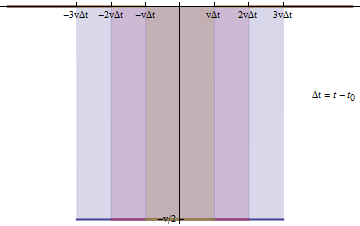
\includegraphics[width=0.5\textwidth]{images/png/for_delta_force.png}
\end{center}

\textbf{Одно тождество}

Рассмотрим функцию вида:
\[
	u(x, t) = \eta(t - t_0) \eta(\xi) f(\xi) = g(\xi, t) f(\xi), \text{ если } \xi = |t - t_0| - |x - x_0|/v 
\]
\[
	\begin{gathered}
	u''_{tt} = 
	\dfs{g}{t} f + 2 \dff{g}{t} \dff{f}{\xi} \dff{\xi}{t} + g \dfs{f}{t} 
	\end{gathered}
\]
\[
	\begin{gathered}
	u''_{xx} = 
	\dfs{g}{x} f + 2 \dff{g}{x} \dff{f}{\xi} \dff{\xi}{x} + g \dfs{f}{x} 
	\end{gathered}
\]
\[
	\begin{gathered}
	u''_{xx} - \frac{1}{v^2} u''_{tt} = 
	f\left(\dfs{g}{x} - \frac{1}{v^2} \dfs{g}{t} \right) + 
	2 \dff{f}{\xi} \dff{g}{\xi} \left[\left(\dff{\xi}{x}\right)^2 - \frac{1}{v^2} \left(\dff{\xi}{t}\right)^2 \right] -
	\frac{2}{v^2} \delta(t - t_0) \eta (\xi) \dff{f}{\xi} \dff{\xi}{t} + 
	\\ +
	g\left[\df{x} \left(\dff{f}{\xi} \dff{\xi}{x} \right) - \frac{1}{v^2} \df{t} \left(\dff{f}{\xi} \dff{\xi}{t} \right)  \right]
	= 
	\\ =
	f\left(\dfs{g}{x} - \frac{1}{v^2} \dfs{g}{t} \right) + 
	2 \dff{f}{\xi} \dff{g}{\xi} \left[\left(\dff{\xi}{x}\right)^2 - \frac{1}{v^2} \left(\dff{\xi}{t}\right)^2 \right] -
	\frac{2}{v^2} \delta(t - t_0) \eta (\xi) \dff{f}{\xi} \dff{\xi}{t} + 
	\\ +
	g\dfs{f}{\xi} \left[\left(\dff{\xi}{x}\right)^2 - \frac{1}{v^2} \left(\dff{\xi}{t}\right)^2 \right] +
	g \dff{f}{\xi} \left(\dfs{\xi}{x} - \frac{1}{v^2} \dfs{\xi}{t} \right)
	\end{gathered}
\]
\[
	\dfs{g}{x} - \frac{1}{v^2} \dfs{g}{t} = - \frac{2}{v} \delta(t - t_0) \delta(x - x_0) \quad \text{(см. пред. пример)}
\]
\[
	\begin{aligned}
	& \dff{\xi}{t} = \sign(t - t_0) & \dff{\xi}{x} = - \sign(x - x_0) \frac{1}{v} \\
	& \dfs{\xi}{t} = 2\delta(t - t_0) & \dfs{\xi}{x} = - 2\delta(x - x_0) \frac{1}{v} \\
	\end{aligned}
\]
\[
	 \begin{gathered}
	 \dff{g}{\xi} \left[\left(\dff{\xi}{x}\right)^2 - \frac{1}{v^2} \left(\dff{\xi}{t}\right)^2 \right] =
	 \eta(t - t_0) \delta(\xi) \frac{1 - 2 \eta(-|x - x_0|) - 1 + 2 \eta(-|t - t_0|)}{v^2} =
	 \\ =
	 \frac{2\eta(t - t_0)}{v^2} (\delta(-|x - x_0|/v) \eta(-|t - t_0|) - \delta(\xi) \eta(-v|t - t_0|) ) = 0
	 \end{gathered}
\]
\[
	\delta(t - t_0) \dff{\xi}{t} = \delta(t - t_0) \sign(t - t_0)  = 0
\]
\[
	\begin{gathered}
	g\left[\left(\dff{\xi}{x}\right)^2 - \frac{1}{v^2} \left(\dff{\xi}{t}\right)^2 \right] =
	\frac{2\eta(t - t_0)}{v^2} (\eta(-|x - x_0|/v) \eta(-|t - t_0|) - \eta(|t - t_0|) \eta(-|x - x_0|) ) =
	\\ =
	- \frac{2\eta(t - t_0)}{v^2} \eta(-|x - x_0|/v) \sign^2(t - t_0)
	\end{gathered}
\]
\[
	\begin{gathered}
	g \left(\dfs{\xi}{x} - \frac{1}{v^2} \dfs{\xi}{t} \right) = 
	- \eta(t - t_0) \eta(\xi) \frac{2}{v^2} \left(\delta((x - x_0)/v) + \delta(t - t_0) \right) =
	\\ =
	- \frac{2}{v^2} \left(\eta^2(t - t_0) \delta((x - x_0)/v) + \frac{1}{2} \eta(-|x - x_0|/v)\delta(t - t_0) \right) =
	\\ =
	- \frac{2}{v^2} \left(\eta(t - t_0) \delta((x - x_0)/v) - \frac{1}{2} \eta(-|t - t_0|) \delta((x - x_0)/v)  + \frac{1}{2} \eta(-|x - x_0|/v)\delta(t - t_0) \right) =
	\\ =
	[\text{чуть выше такое уже встречалось}] =
	- \frac{2}{v} \eta(t - t_0) \delta(x - x_0)
	\end{gathered}
\]
В результате:
\[
	u''_{xx} - \frac{1}{v^2} u''_{tt}  = - \frac{2}{v} f(0) \delta(t - t_0) \delta(x - x_0) -
	f''(|t - t_0|) \frac{\eta(t - t_0)}{v^2} \sign^2(t - t_0) \eta(-|x - x_0|) -
	\frac{2}{v} f'(|t - t_0|) \eta(t - t_0) \delta(x - x_0)
\]

Здесь следует отметить одну деталь: результат имеет вид:
\[
	A\delta(x) + B\eta(-|x|)
\]
Из интегрального определения $\delta-$функции:
\[
	A\delta(x) + B\eta(-|x|) = A\delta(x)
\]
И
\[
	u''_{xx} - \frac{1}{v^2} u''_{tt}  = - \frac{2}{v} f(0) \delta(t - t_0) \delta(x - x_0) -
	\frac{2}{v} f'(|t - t_0|) \eta(t - t_0) \delta(x - x_0)
\]

\textbf{2. Пусть:}
\[
s(x, t) = \delta(x - x_0) \eta(t - t_0)
\]
что соответствует постоянной во времени силе, действующей в фиксированной точке струны, начиная с некоторого момента.
\[
\begin{gathered}
u(x, t) =
-\frac{v}{4} \int\limits_{0}^{t} \! \int\limits_{-\infty}^{\infty} [ \sign (\xi + v \tau) - \sign (\xi - v\tau) ]  \delta(x - x_0 - \xi) \eta(t - t_0 - \tau) d\tau d\xi =
\\ =
-\frac{v}{4} \int\limits_{0}^{t} [ \sign (x - x_0 + v \tau) - \sign (x - x_0 - v\tau) ] \eta (t - t_0 - \tau)  d\tau =
\\ =
-\frac{v}{4} \eta(t - t_0) \int\limits_{0}^{t - t_0} [ \sign (x - x_0 + v \tau) - \sign (x - x_0 - v\tau) ] d\tau = 
-\frac{v}{4} \eta(t - t_0) \int\limits_{0}^{t - t_0} 2 \eta(v|\tau| - |x - x_0|) d\tau =
\\ =
-\frac{v}{4} \eta(t - t_0) \eta(t - t_0 - |x - x_0|/v) \int\limits_{|x - x_0|/v}^{t - t_0} 2 \eta(v\tau - |x - x_0|) d\tau = 
-\frac{v}{2} \eta(t - t_0) \eta(t - t_0 - |x - x_0|/v) \int\limits_{|x - x_0|/v}^{t - t_0} d\tau =
\\ =
-\frac{v}{2} \eta(t - t_0) \eta(t - t_0 - |x - x_0|/v) (t - t_0 - |x - x_0|/v) 
\end{gathered}
\]
Проверка по формуле выше показывает, что это правильный ответ. Форма струны в различные моменты времени показана на рисунке:
\begin{center}
	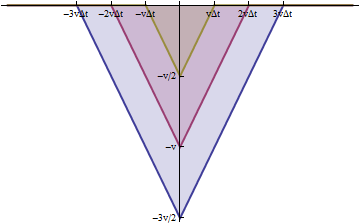
\includegraphics[width=0.5\textwidth]{images/png/for_deltac_force.png}
\end{center}

\textbf{3. Пусть:}
\[
	s(x, t) = \begin{cases}
	0, & x \notin [-l/2, l/2] \\
	S_0\eta(t - t_0)/l, & x \in [-l/2, l/2]
	\end{cases} =
	\frac{S_0}{l} [ \eta(x + l/2) - \eta(x - l/2)] \eta(t - t_0)
\]
что соответствует постоянной силе, действующей на участок струны.
\[
\begin{gathered}
	u(x, t) =
	-\frac{v}{2} \int\limits_{0}^{t} \! \int\limits_{-v\tau}^{v\tau} s(x - \xi, t - \tau) d\tau\, d\xi = 
	\\ =
	-\frac{v}{2} \int\limits_{0}^{t} \! \int\limits_{-v\tau}^{v\tau} \frac{S_0}{l} [ \eta(x + l/2 - \xi) - \eta(x - l/2 - \xi)]\eta(t - t_0 - \tau) d\tau\, d\xi = 
	\\ =
	-\frac{v}{2} \int\limits_{0}^{t - t_0} \! \int\limits_{-v\tau}^{v\tau} \frac{S_0}{l} [ \eta(x + l/2 - \xi) - \eta(x - l/2 - \xi)] d\tau\, d\xi = 
	-\frac{v}{2}\frac{S_0}{l} \int\limits_{S} d\tau\, d\xi
\end{gathered}
\]
Область интегрирования $S$ приведена на рисунке, и представляет собой пересечение полосы шириной $l$ и треугольника, ограниченного кривыми $y = v(t - t_0)$, $y = x$, $y = -x$.
\begin{center}
	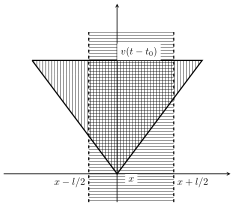
\includegraphics{images/png/for_example3.png}
	%\usetikzlibrary{patterns}
\begin{tikzpicture}

\draw[thick,-stealth]  (0,-1) -- (0,6);
\draw[thick,-stealth] (-4,0) -- (4,0);
\draw[very thick, pattern=vertical lines] (-3,4) -- (3, 4) -- (0,0) -- (-3, 4);
\draw[very thick, dashed] (2, -1) -- (2, 5);
\draw[very thick, dashed] (-1, -1) -- (-1, 5);
\path[pattern=horizontal lines] (2, -1) rectangle (-1, 5);

\node[below, fill = white] at (0.5,0) {$x$};
\node[above right, fill = white] at (0,4) {$v(t - t_0)$};
\node[below left] at (-1,0) {$x - l/2$};
\node[below right] at (2,0) {$x + l/2$};

\end{tikzpicture}
\end{center}
Решение можно представить с помощью функций, определяющих площадь пересечения треугольника с левой полуплоскостью, заданной прямой параллельной оси ординат:
\[
\begin{aligned}
& S_+(x, x_A, x_B, x_C, y_B) =  
\frac{1}{2} y_B \frac{(x - x_A)^2}{x_B - x_A} \eta(x - x_A) \eta(x_B - x)  + \\ & +
\frac{1}{2} y_B \left[(x_B - x_A) + \frac{2 x_C - x - x_B}{x_C - x_B} (x - x_B)\right] \eta(x - x_B) \eta(x_C - x) +
\frac{1}{2} y_B (x_C - x_A) \eta(x - x_C)
\end{aligned}
\]
\[
	\begin{aligned}
	u(x, t) & = -\frac{v}{2}\frac{S_0}{l} [S_+(x + l/2, -v(t - t_0), 0, v(t-t_0), v(t - t_0)) - S_+(x - l/2, -v(t - t_0), 0, v(t-t_0), v(t - t_0))]
	\end{aligned}
\]
К сожалению, выражение слишком громоздко, и его трудно проверить. На рисунке приведена форма струны в различные моменты времени:
\begin{center}
	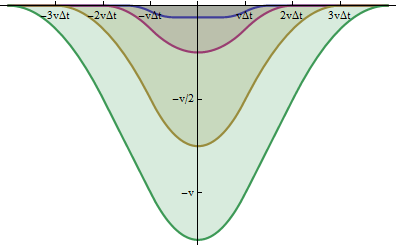
\includegraphics[width=0.5\textwidth]{images/png/for_const_force.png}
\end{center}
Примечательно, что сначала график пологий, но со временем приобретает более параболическую форму.

\textbf{4. Пусть:}

\[
s(x, t) = \delta(x - x_0) e^{i\omega t} \eta(t - t_0)
\]
что соответствует силе действующей в точке по синусоидальному закону.
\[
\begin{gathered}
u(x, t) =
-\frac{v}{4} \int\limits_{0}^{t} \! \int\limits_{-\infty}^{\infty} [ \sign (\xi + v \tau) - \sign (\xi - v\tau) ] s(x - \xi, t - \tau) d\tau d\xi =
\\ =
-\frac{v}{4} \int\limits_{0}^{t} \! \int\limits_{-\infty}^{\infty} [ \sign (\xi + v \tau) - \sign (\xi - v\tau) ] \delta(x - x_0 - \xi) e^{i\omega(t - \tau)} \eta(t - t_0 - \tau) d\tau d\xi =
\\ =
-\frac{v}{2} \eta(t - t_0) \int\limits_{0}^{t - t_0} \eta(v\tau - |x - x_0|) e^{i\omega(t - \tau)} d\tau =
-\frac{v}{2} \eta(t - t_0) \eta(t - t_0 - |x -x_0|/v) e^{i\omega t} \int\limits_{|x - x_0|/v}^{t - t_0} e^{-i\omega\tau} d\tau =
\\ =
\frac{v}{2i\omega} \eta(t - t_0) \eta(t - t_0 - |x -x_0|/v) e^{i\omega t} e^{-i\omega(t - t_0 - |x - x_0|/v)} =
\frac{v}{2i\omega} \eta(t - t_0) \eta(t - t_0 - |x -x_0|/v) \left(e^{i\omega t_0} - e^{i\omega(t - |x - x_0|/v)} \right)
\end{gathered}
\]
Как легко видеть, ответ правильный. Действительная часть:
\[
	u(x, t) = \frac{v}{2\omega} \eta(t - t_0) \eta(t - t_0 - |x -x_0|/v) \left(\sin (\omega t_0) - \sin(\omega(t - |x - x_0|/v)) \right)
\]
Форма в различные моменты времени представлена на рисунке:
\begin{center}
	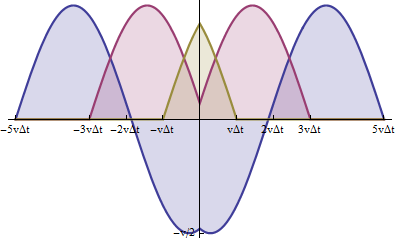
\includegraphics[width=0.5\textwidth]{images/png/for_sin_force.png}
\end{center}

\subsection{Вариационный принцип}

Рассмотрим функционал:
\[
	J(u) = \int\limits_{R^2} \left[\frac{1}{v^2} \left(\dff{u}{t}\right)^2 - \left(\dff{u}{x}\right)^2 \right] dx\, dt  
\]
\[
	\begin{gathered}
	\delta \left[\frac{1}{v^2} \left(\dff{u}{t}\right)^2 - \left(\dff{u}{x}\right)^2 \right] = 
	2 \left[\frac{1}{v^2} \dff{u}{t} \dff{\delta u}{t}  - \dff{u}{x} \dff{\delta u}{x} \right] =
	2 \left[\frac{1}{v^2} \df{t} \left(\dff{u}{t} \delta u \right)  - \df{x} \left(\dff{u}{x} \delta u \right) \right] -
	2 \left[\frac{1}{v^2} \dfs{u}{t} - \dfs{u}{x}\right] \delta u
	\end{gathered}
\]
\[
	\Rightarrow \quad \frac{1}{v^2} \dfs{u}{t} - \dfs{u}{x} = 0
\]
Для функционала:
\[
	J(u) = \int\limits_{R^2} \left[\frac{1}{v^2} \left(\dff{u}{t}\right)^2 - \left(\dff{u}{x}\right)^2 - 2 s(x, t) u \right] dx\, dt
\]
\[
	\frac{1}{v^2} \dfs{u}{t} - \dfs{u}{x} = s(x, t)
\]
Выполним преобразование Фурье:
\[
	u = u^* = \int\limits_{R^2} U(k, \omega) e^{i(\omega t - k x)} dk\, d\omega
	\qquad
	s = s^* = \int\limits_{R^2} S(k, \omega) e^{i(\omega t - k x)} dk\, d\omega
\]
\[
	\begin{gathered}
	J(U) = 
	\\ =
	\int\limits_{R^2} 
	\int\limits_{R^2}
	\int\limits_{R^2}
	\left[\frac{1}{v^2} \omega \omega' U^*(k, \omega) U(k', \omega') - k k' U^*(k, \omega) U(k', \omega') - 2 S^*(k, \omega) U(k', \omega') \right]
	e^{i((\omega' - \omega) t - (k' - k) x)}  dk\, d\omega\, dk'\, d\omega'\, dx\, dt
	=
	\\ =
	2\pi 
	\int\limits_{R^2} 
	\int\limits_{R^2}
	\left[\frac{1}{v^2} \omega \omega' U^*(k, \omega) U(k', \omega') - k k' U^*(k, \omega) U(k', \omega') - 2 S^*(k, \omega) U(k', \omega') \right]
	\delta(\omega' - \omega) \delta(k' - k) dk\, d\omega\, dk'\, d\omega'
	=
	\\ =
	2\pi 
	\int\limits_{R^2} 
	\left[\frac{1}{v^2} \omega^2 U^*(k, \omega) U(k, \omega) - k^2 U^*(k, \omega) U(k, \omega) - 2 S^*(k, \omega) U(k, \omega) \right]
	dk\, d\omega
	\end{gathered}
\]

\subsection{Решение n-мерного волнового уравнения с дельтообразной правой частью}

Волновое уравнение с дельтообразной правой частью в бесконечном пространстве-времени чудесная вещь:
\[
	\Delta u - \frac{\partial^2 u}{\partial t^2} = \delta(t - t')\delta(\vec{r} - \vec{r}') 
\]
Выполняем преобразование Фурье:
\[
	u = \int U(\vec{k}, \omega) e^{i(\vec{k}\cdot\vec{r} - \omega t)} dV_k dt
\]
Введём обозначения:
\[
	\vec{R} = \vec{r} - \vec{r}' \quad T = t - t'
\]
\[
	\delta(\vec{R}) \delta(T) = \frac{1}{(2\pi)^{n + 1}} \int e^{i(\vec{k}\cdot\vec{R} - \omega T)} dV_k d\omega
\]
Решение уравнения:
\[
	u = \frac{1}{(2\pi)^{n + 1}} \int \frac{e^{i(\vec{k}\cdot\vec{R} - \omega T)}}{\omega^2 - k^2} dV_k d\omega =  
	\frac{\pi^{(- n - 3)/2}}{2^n\Gamma\left(\frac{n - 1}{2}\right)} 
	\int\limits_{-\infty}^{\infty}\!
	\int\limits_{0}^{\infty}\!
	\int\limits_{0}^{\pi}
	 \frac{e^{i(k R \cos \theta - \omega T)}}{\omega^2 - k^2} k^{n - 1} \sin^{n - 2} \theta\, d\theta\, dk\, d\omega = (*)
\]
\[
	\frac{1}{\omega^2 - k^2} = \frac{1}{2k} \left(\frac{1}{\omega - k} - \frac{1}{\omega + k} \right)
\]
\[
	\begin{gathered}
	(*) =
	\frac{i \pi^{(- n - 1)/2}}{2^{n + 1}\Gamma\left(\frac{n - 1}{2}\right)} 
	\int\limits_{0}^{\infty}\!
	\int\limits_{0}^{\pi}
	\left(e^{ - i k T}  - e^{i k T} \right) \sign(-T)
	e^{i(k R \cos \theta)} 
	k^{n - 2} \sin^{n - 2} \theta\, d\theta\, dk
	= \\ =
	\frac{\pi^{(- n - 1)/2}}{2^{n}\Gamma\left(\frac{n - 1}{2}\right)} 
	\int\limits_{0}^{\infty}\!
	\int\limits_{0}^{\pi}
	\sin (kT) \sign(-T)
	e^{i(k R \cos \theta)} 
	k^{n - 2} \sin^{n - 2} \theta\, d\theta\, dk
	\end{gathered} 
\]